\documentclass[uplatex, onecolumn, 10pt]{jsarticle}

\usepackage[dvipdfmx]{graphicx}
\usepackage{latexsym}
\usepackage{bmpsize}
\usepackage{url}
\usepackage{comment}
\usepackage{ulem}
\usepackage{amssymb}

\def\Underline{\setbox0\hbox\bgroup\let\\\endUnderline}
\def\endUnderline{\vphantom{y}\egroup\smash{\underline{\box0}}\\}

\newcommand{\ttt}[1]{\texttt{#1}}

\begin{document}

\title{\vspace{-40mm}\bf{\LARGE{ゼミ報告書}}}
\author{\vspace{-40mm}木村 優哉  T2401199}
\date{1900-01-01 Mon}
\maketitle


\section{今日までにやったこと}

\subsection*{研究関連}
\begin{itemize}
	\item 英論翻訳
	\item 先輩の卒論・修論拝読
	\begin{itemize}
        \item $\bigcirc \bigcirc$ さんの卒論(タイトル $\times \times$ )
        \item 本当は $\uparrow$ みたいに \LaTeX の記号使わないけどね
    \end{itemize}
\end{itemize}

\subsection*{その他}
\begin{itemize}
	\item バイト関連
	\item ロボコン関連
	\item マウス買った、キーボード買ったなどのことも書いていいよ
\end{itemize}



\section{次までにやること}

\subsection*{研究関連}
\begin{itemize}
	\item 関連研究調査
    \item 卒論執筆
	\item 修論執筆
\end{itemize}

\subsection*{その他}
\begin{itemize}
	\item バイト関連
	\item ロボコン関連
	\item ゼミ報告書の環境を移行する
\end{itemize}

\newpage

\begin{figure}[t]
    \begin{center}
        \fbox{
            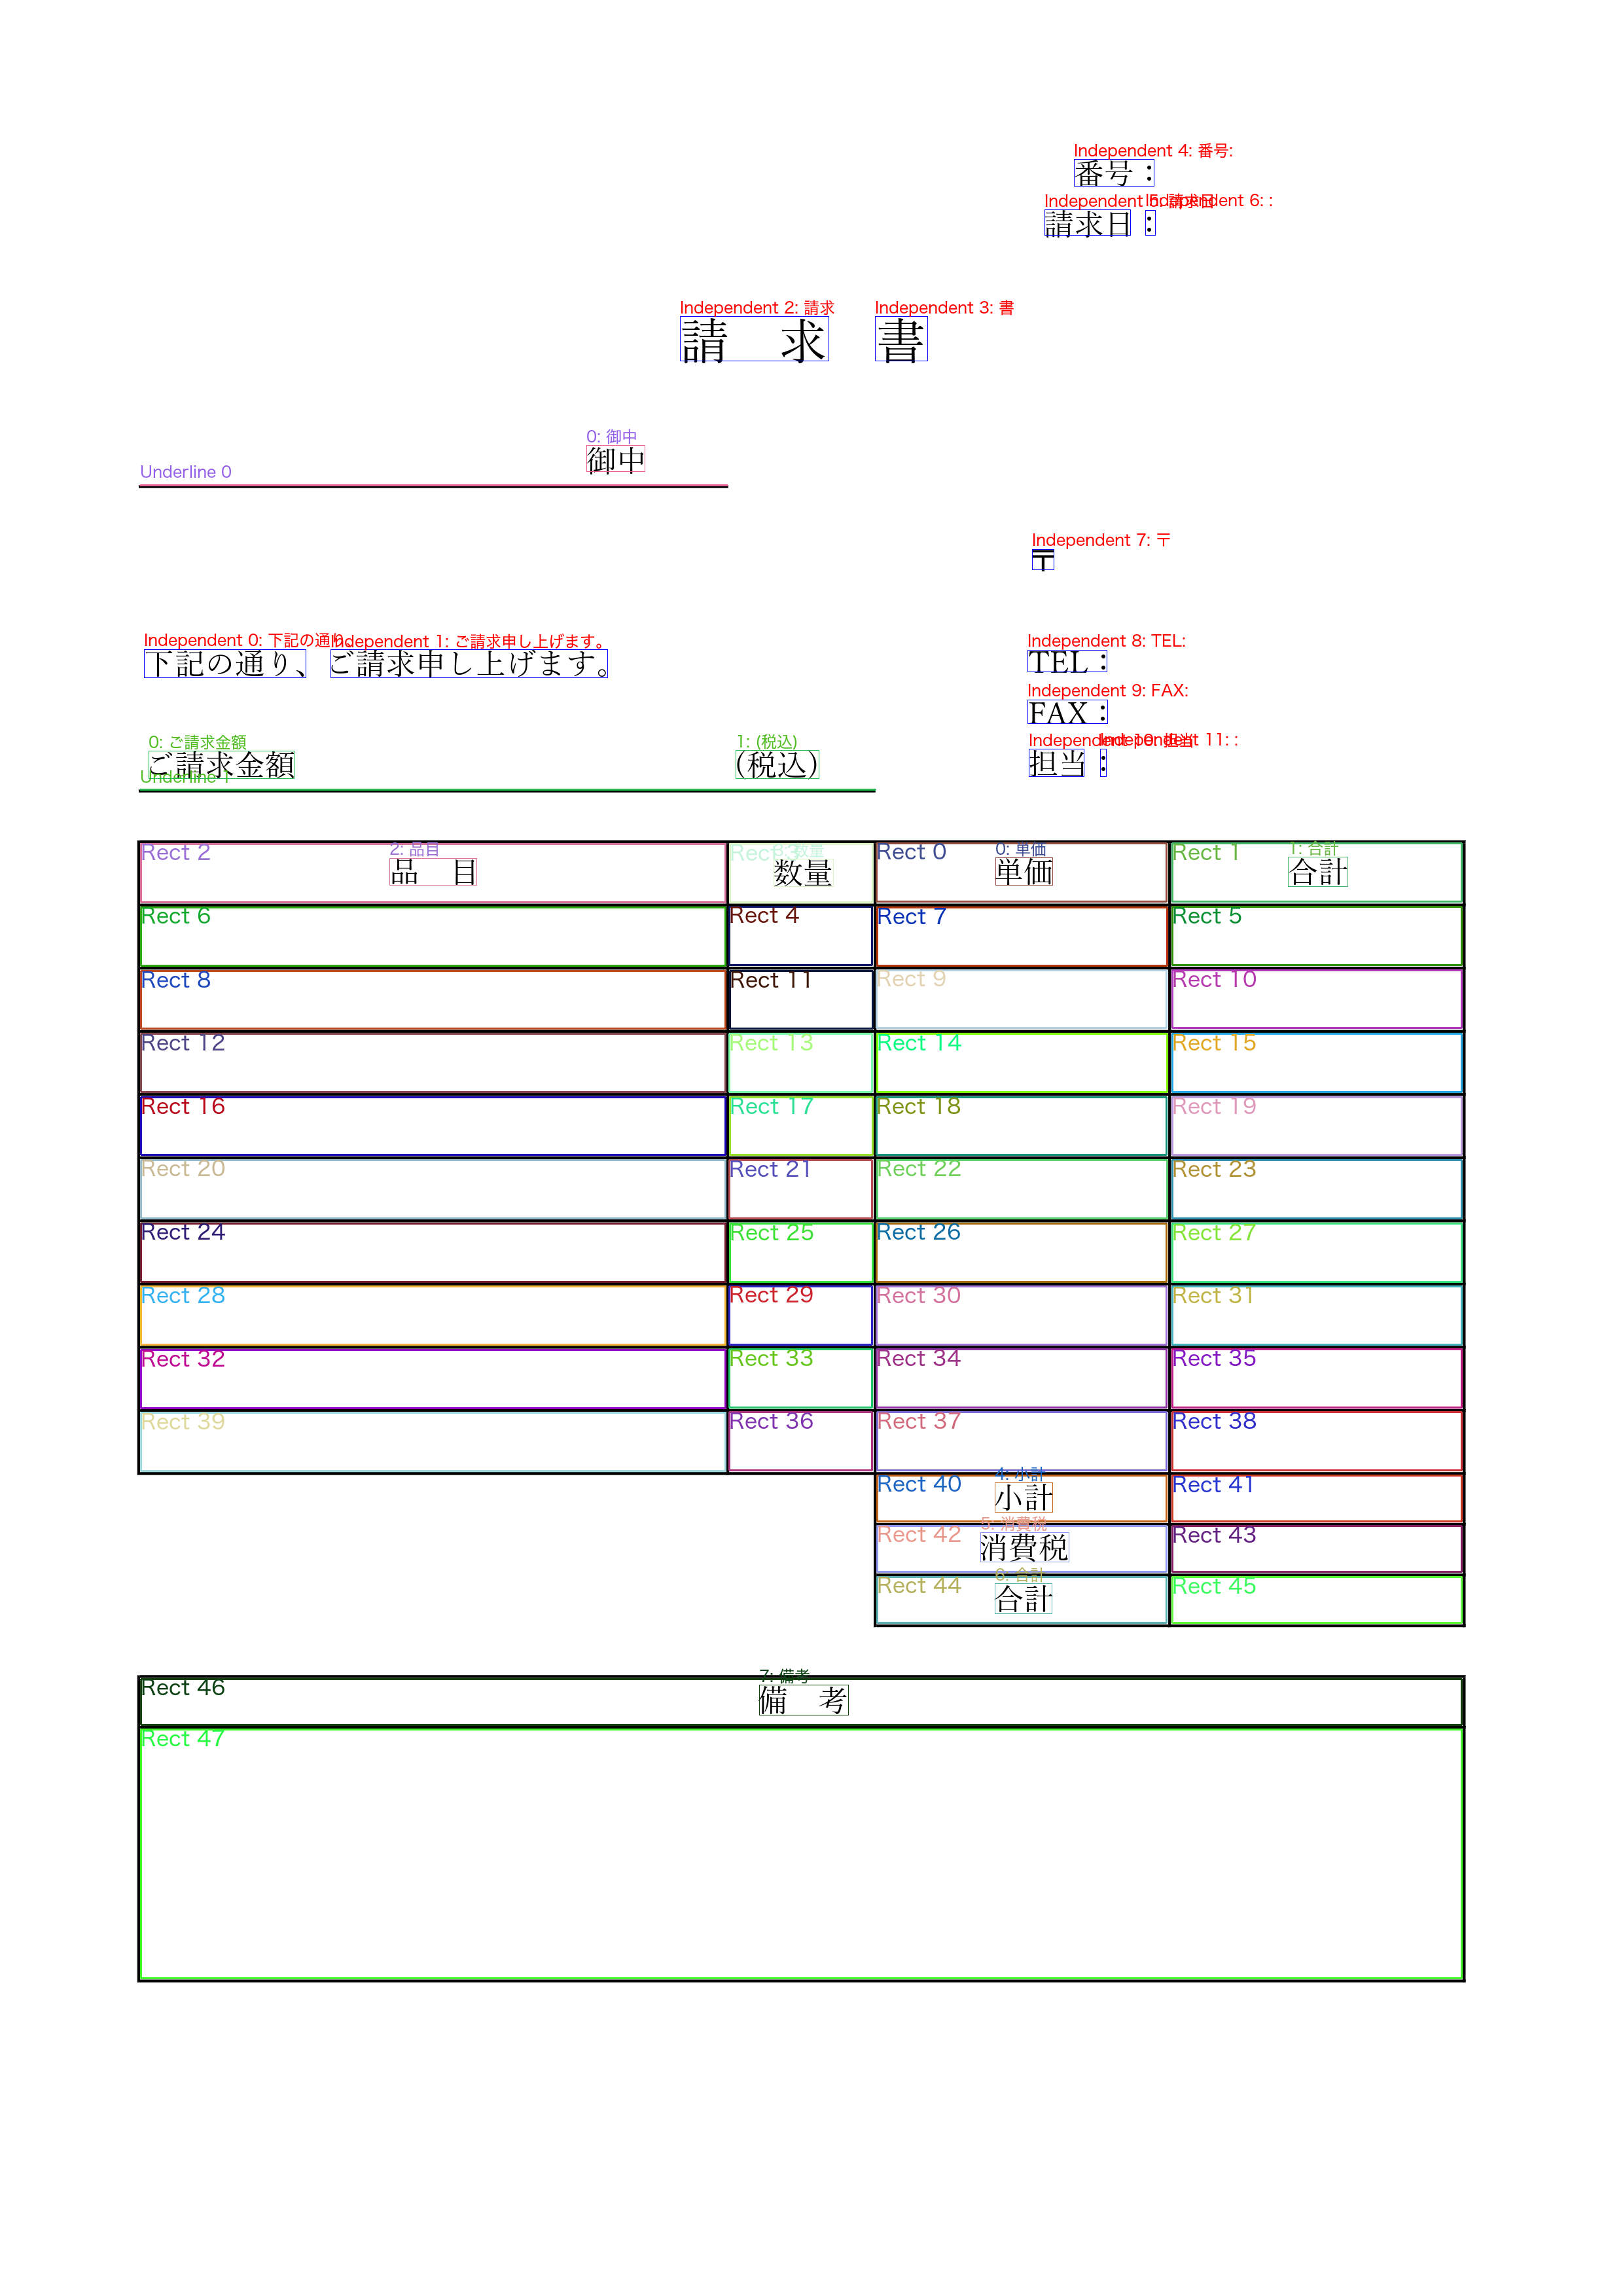
\includegraphics[keepaspectratio,width=0.4\linewidth]{image/image_linked.png}
            }
            \caption{こんな感じで画像も置けるよ}
    \end{center}
\end{figure}

\begin{figure}[t]
    \begin{center}
        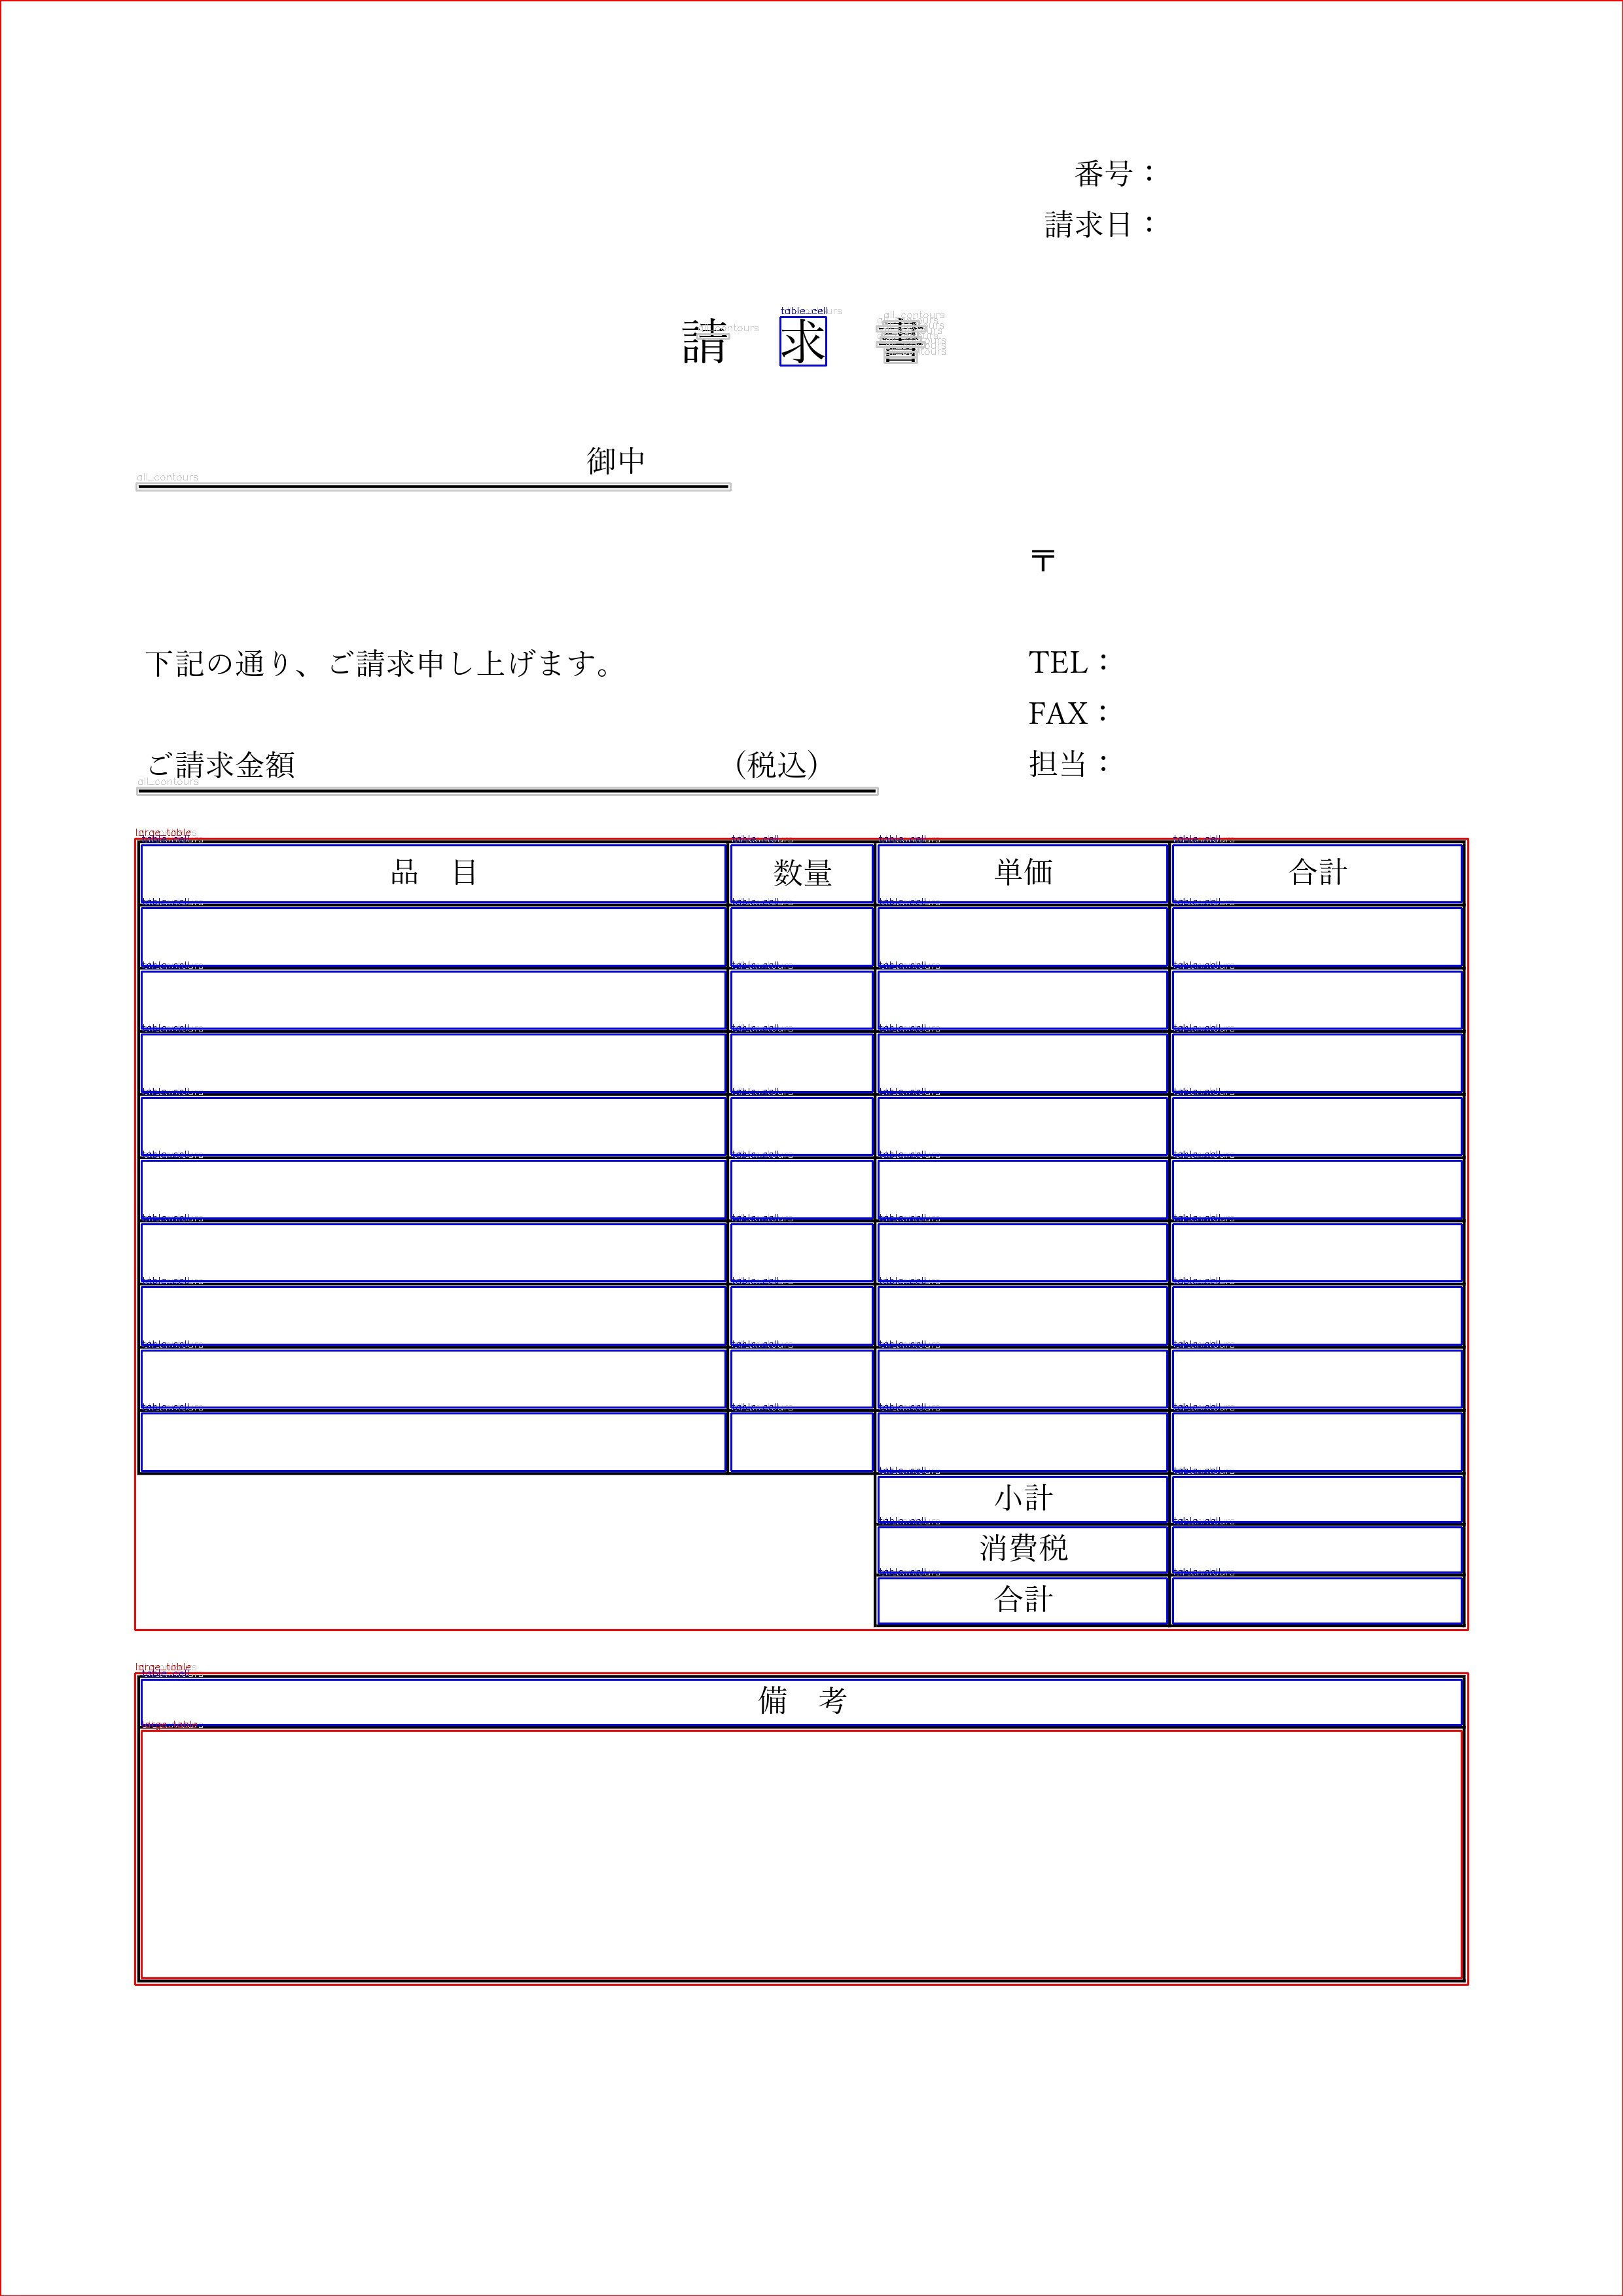
\includegraphics[keepaspectratio,width=0.4\linewidth]{image/seikyuu_rectangles.jpg}
        \caption{\textbackslash newpage で次ページに置けるよ}
    \end{center}
\end{figure}

\end{document}
